\section{Background}
\subsection{2023-2024 - Borealis}
\label{test}
The rocket Borealis was Waterloo Rocketry's first attempt at flying (and for all intents and purposes, developing) active control systems, in the form of airbrakes. At the outset of the airbrakes project, it was envisioned that a working group would develop something like Figure \ref{fig:ab-model}.

\begin{figure}[ht]
    \centering
    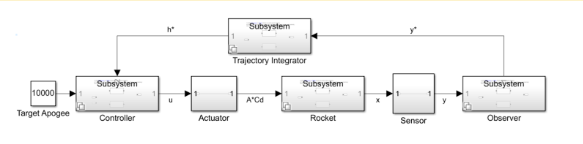
\includegraphics[width=0.8\linewidth]{images/airbrakes.png}
    \caption{Airbrakes control loop structure}
    \label{fig:ab-model}
\end{figure}

Everything except "Actuator" and "Rocket" were implemented to some degree in the final flight software, but Simulink was never actually used other than to create the above diagram.

A PID controller was ultimately selected for airbrakes because the team lacked the knowledge and scope for anything more complex. This controller was "tuned" using a plugin for OpenRocket (OR) \cite{or-brake}, dynamically modifying the drag force used by OR in its calculations with values produced from external computational fluid dynamics simulations. Later versions included the ability to inject random noise into the state measurements. Under these noisy conditions, simulations suggested the controller could get within about 20m of the target altitude over most of the controllable regime (20,000 +/- 2,000 ft.). 

While much more useful at the time than having no controller-in-loop simulation options at all, the OR plugin was not sustainable. The overlap between Waterloo Rocketry members (and budding control engineers) and Java developers was and still is very small. The final plugin version ran the controller as a binary compiled from the same C source code as the board on the rocket, and while this was also a promising development in the team's testing practices, the process for doing this was even less accessible than running the plugin itself. The plugin project was ultimately an uphill battle to turn OR into something it wasn't meant to be. This motivated the development of a complete simulation alternative in Simulink which could be effectively used for estimator/controller development and validation.

\subsection{Project Jupiter}
Projeto Jupiter is a rocketry team from the University of São Paulo, Brazil. They conveniently already developed most of what is necessary for a plant model of a sounding rocket with canards in Simulink \cite{jupiter-canards}. Rather than trying to start more or less from scratch as it was planned last year, the goal this year was essentially to modify their plant model with our rocket design parameters, verify it for uncontrolled flight against the OR baseline, and then begin simulating the effects of canards.

\section{Theory}
Compared to a dynamic model of a real launch vehicle, a sounding rocket is considerably simpler. In particular, sloshing, bending, and TVC dynamics do not need to be considered. The rocket can be treated as a single rigid body with time-varying mass and mass distribution. The only forces acting on an uncontrolled rocket are engine thrust, gravity, and drag. Of these, gravity applies no moment by definition, and the moment applied by thrust, due to misalignment with the rocket centre of mass, is constant and typically negligible. Since gravity is well defined and engine thrust is defined empirically via propulsion test data, this leaves the aerodynamic forces and moments as the most complicated aspect of simulation.

Barrowman provides empirical methods for computing the centre of pressure of a rocket's components at relatively low Mach numbers. (link FD docs). The coefficient of drag ($C_d$) is modelled only as a function of Mach number for a given rocket, using either OR or RASAero data. In the future, other drag models may be considered.

\section{Implementation}
All units are SI - MKS, with the exception of the sensor interface (see below), which uses output units matching the physical IMUs they represent. Due to restrictions of certain blocks, the WGS84 earth model is used where applicable.

\subsection{Simulation Setup}
A rocket-specific script (e.g. borealis.m) imports a CSV file from OR containing relevant data. This script also hard-codes the geometric parameters like reference length, fin location, etc. which OR does not export. The script performs additional post-processing on the data as necessary, including differentiating the mass over time and converting the $C_d$/Mach time series into a direct lookup. A generic post-processing script transforms the rocket data into the format the simulation expects. Together, it is possible to simulate any rocket given input geometry and simulation export from OR.

The OR wind model has not been investigated, and so all OR data is supplied for the no wind case.

\subsection{Top Level Plant}
The plant model is composed of three subsystems: the canards actuator, the rocket flight dynamics, and the sensors. Figure \ref{fig:plant-model} shows the connection of these subsystems. A visualization subsystem plots the output values of the flight dynamics against the OR results for validation purposes.

\begin{figure}[ht]
    \centering
    
\includegraphics[width=0.9\linewidth]{images/top_level_plant.png}
    \caption{Canards Plant Model Interface}
    \label{fig:plant-model}
\end{figure}

\subsection{Actuator}
The actuator is modelled as a nonlinear second-order system with deadband to account for internal backlash. This is in contrast to the linear first-order model used by the estimator.  

\begin{figure}[ht]
    \centering
    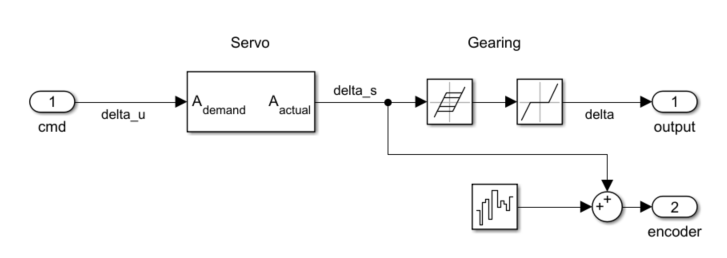
\includegraphics[width=0.75\linewidth]{images/actuator.png}
    \caption{Canards Actuator Dynamics}
    \label{fig:actuator-dynamics}
\end{figure}

\subsection{Rocket Flight}
\subsubsection{6DOF Variant Mass Model}
The core of the plant model is the "Simple Variable Mass 6DOF" block provided by the Aerospace Blockset. It takes in net force and moment about the center of mass at each time step and outputs translational and rotational position and velocity.
Note that the inputs are provided in the body fixed frame, with the X axis coincident with the longitudinal axis of the rocket body. The translational position and velocity are provided in the flat earth reference frame. The origin of this inertial frame is arbitrary for dynamics purposes, but is effectively the position of the launch rail on the earth surface.
The 6DOF block does not output mass vs time, instead providing inputs for starting mass, ending mass, and a $\frac{dm}{dt}$. The starting and ending moment of inertia are interpolated between using $\frac{dm}{dt}$.

%\subsubsection{Wind Model}
%The wind simulation operates similar to Niskanen [cite?]. The winds take on a constant speed at all altitudes, with pink noise for turbulence added on top. This turbulence is also responsible for any and all rotational speed of the wind. Additionally, gusting has been added on top of the base wind model, which allows for gusts of set strength and direction to happen after a specified time. Similar to OR, the simulation takes a user-input base wind velocity, base wind direction, and turbulence value. The user must also specify the magnitude, time of occurrence, and duration of gusts.

\subsubsection{Roll Dynamics}
The two rocket components which affect roll are the fins and canards. For roll dynamics, they are split into separate parts and treated independently. This allows the canards to be handled with more detail or with different aerodynamic models if needed.

For the fins, the aerodynamic coefficients and derivatives are calculated using Barrowman's equations and then fed into the Simulink model. This is done by the "roll forcing and damping block" in the plant. The only significant change from an aerodynamics standpoint is the mach-speed correction term on the coefficients, which is normally taken to be $$ \mathcal{B}^{-1} = \frac{1}{\sqrt{\lvert 1-M^2 \rvert}}$$

Since this breaks at $M = 1$ and it is commonly held that it peaks at around 2 near sonic speeds, we take $\mathcal{B}$ to be the minimum of the above expression and 2.

\subsubsection{Pitch Dynamics}
The methodology used to compute the normal force components which affect pitch dynamics is the same as that of OR \cite{or-manual} (see Sec. 3.2.1). The rocket body is divided into its components: nosecone, body, fin, tail, and canards (if applicable). The local velocity of the rocket at the component centre of pressure, relative to the wind, is computed and along with the component $C_{N_\alpha}$ is used to compute the normal force and moment vectors. This functionality is encapsulated in a generic "lift component" block, whose internals are shown in Fig \ref{fig:lift-component}:
\begin{figure}[ht]
    \centering
    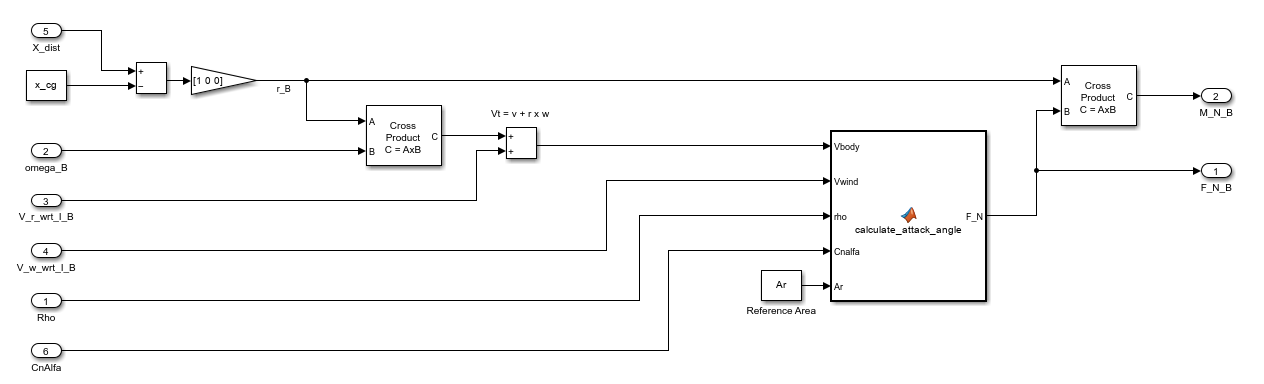
\includegraphics[width=0.9\linewidth]{images/lift_comp.png}
    \caption{Lift Component subsystem}
    \label{fig:lift-component}
\end{figure}

These blocks are composed to calculate the net normal force and moment:
\begin{figure}[ht]
    \centering
    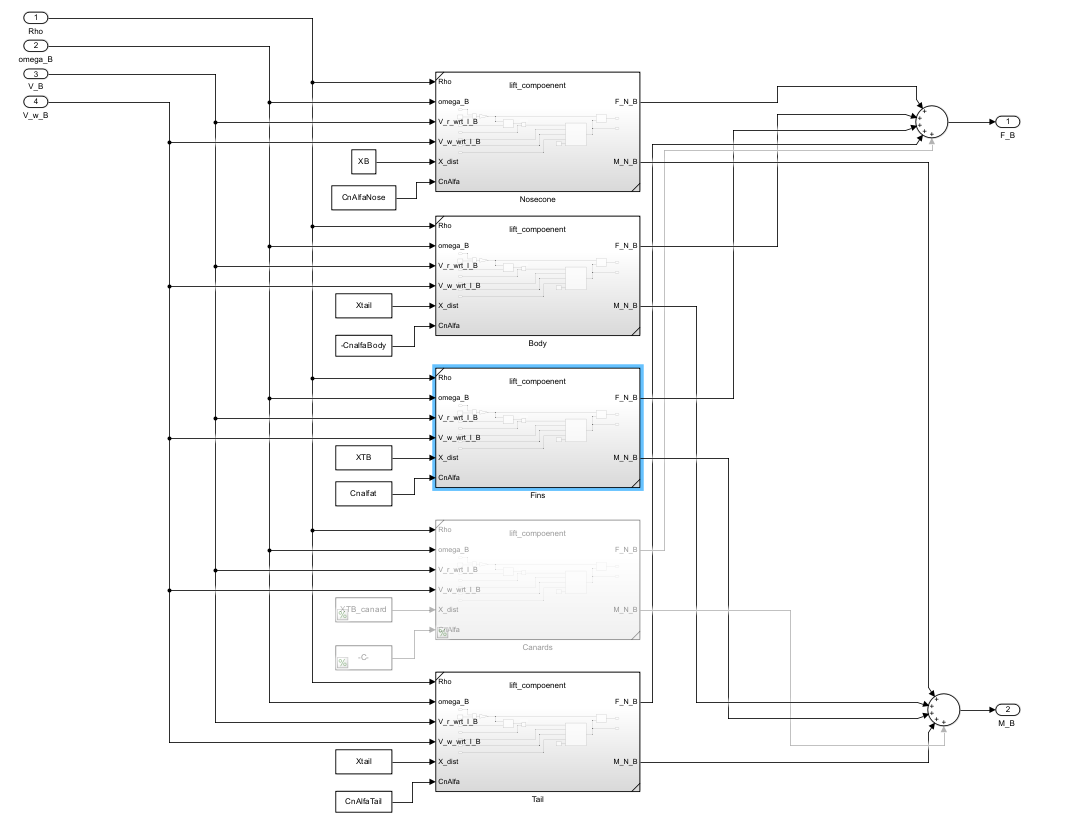
\includegraphics[width=0.9\linewidth]{images/normal_force.png}
    \caption{Normal Force and Moment}
    \label{fig:normal-force}
\end{figure}

\subsection{Sensors}
In order to test the robustness of the controller to real-world sensor outputs, the IMU (accelerometer, gyroscope), magnetometer, and barometer (only pressure) outputs are simulated, adding noise and bias. This is done through custom MatLab scripts that track drift over the simulation and continuously add it to the measured quantities. 

The estimator is connected to 3 unlike IMUs for redundancy, and to alleviate saturation. The Movella MTi-630 is an integrated Altitude and Heading Reference System (AHRS), which contains its own onboard orientation filter. The LSM6DSV32X and AltIMU-10 are an IMU and IMU carrier board respectively. They are henceforth all referred to as "IMUs". In the final implementation, data is sampled from all IMUs at the nominal execution rate, concatenated, and passed to the estimator for processing. In order to simulate the dynamics of each IMU, a custom IMU component is defined (\ref{fig:imu-component}).

\begin{figure}[ht]
    \centering
    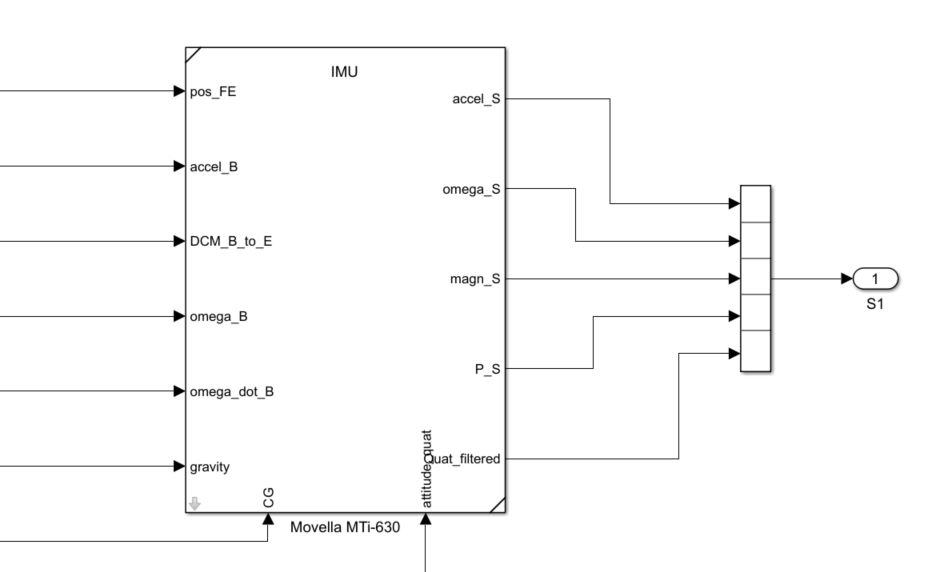
\includegraphics[width=0.9\linewidth]{images/imu_movella.png}
    \caption{Standard IMU Component Instance for Movella MTi-630}
    \label{fig:imu-component}
\end{figure}

